% !TEX TS-program = pdfLaTeX+MakeIndex+BibTeX
% !TEX encoding = UTF-8 Unicode

\PassOptionsToPackage{unicode}{hyperref}
\PassOptionsToPackage{naturalnames}{hyperref}

\documentclass[tg]{mdtufsm}

\usepackage[T1]{fontenc}
\usepackage{fix-cm}
\usepackage{url}
\usepackage{times, color}
\usepackage[utf8]{inputenc}
\usepackage{graphicx}
\usepackage{amsmath,latexsym,amssymb}
%\usepackage[hidelinks]{hyperref}
\usepackage[hidelinks,
            bookmarksopen=true,linktoc=none,colorlinks=true,
            linkcolor=black,citecolor=black,filecolor=magenta,urlcolor=blue,
            pdftitle={Um sistema web para execução remota de aplicações de alto desempenho},
            pdfauthor={Otávio Migliavacca Madalosso},
            pdfsubject={Trabalho de Graduação},
            pdfkeywords={Computação de alto desempenho, programação web, Framework Django,  Execução Remota, Informática, UFSM}
            ]{hyperref}
            
%\usepackage[brazilian]{babel}

%\usepackage{fontspec}
%\setmainfont{Linux Libertine G}

%%% PAGE DIMENSIONS
\usepackage[inner=30mm,outer=20mm,top=30mm,bottom=20mm]{geometry} 
\usepackage{epstopdf}
\usepackage{graphicx}
\usepackage{pdfpages}
% \geometry{margin=2in} % for example, change the margins to 2 inches all round
% \geometry{landscape} % set up the page for landscape

% \usepackage[parfill]{parskip} % Activate to begin paragraphs with an empty line rather than an indent

%%% PACKAGES
%\usepackage{amsfonts}
\usepackage{color}
%\usepackage{booktabs} % for much better looking tables
%\usepackage{array} % for better arrays (eg matrices) in maths
%\usepackage{paralist} % very flexible & customisable lists (eg. enumerate/itemize, etc.)
\usepackage{verbatim} % adds environment for commenting out blocks of text & for better verbatim
\usepackage{listings}
\usepackage{parcolumns}
\usepackage{siunitx}
%\usepackage{verbatim} % adds environment for commenting out blocks of text & for better verbatim
\usepackage{subcaption}
\captionsetup{compatibility=false}
%\usepackage{microtype}
%\usepackage[numbers]{natbib}
%\usepackage{subfig} % make it possible to include more than one captioned figure/table in a single float
% These packages are all incorporated in the memoir class to one degree or another...

\definecolor{codegreen}{rgb}{0,0.6,0}
\definecolor{codegray}{rgb}{0.5,0.5,0.5}
\definecolor{codepurple}{rgb}{0.58,0,0.82}
\definecolor{backcolour}{rgb}{0.95,0.95,0.92}
\lstdefinestyle{mystyle}{
	backgroundcolor=\color{backcolour},   commentstyle=\color{codegreen},
	keywordstyle=\color{magenta},
	numberstyle=\tiny\color{codegray},
	stringstyle=\color{codepurple},
	basicstyle=\footnotesize,
	breakatwhitespace=false,         
	breaklines=true,                 
	captionpos=b,                    
	keepspaces=true,                 
	numbers=left,                    
	numbersep=5pt,                  
	showspaces=false,                
	showstringspaces=false,
	showtabs=false,                  
	tabsize=2,
	literate=
	{á}{{\'a}}1 {é}{{\'e}}1 {í}{{\'i}}1 {ó}{{\'o}}1 {ú}{{\'u}}1
	{Á}{{\'A}}1 {É}{{\'E}}1 {Í}{{\'I}}1 {Ó}{{\'O}}1 {Ú}{{\'U}}1
	{à}{{\`a}}1 {è}{{\`e}}1 {ì}{{\`i}}1 {ò}{{\`o}}1 {ù}{{\`u}}1
	{À}{{\`A}}1 {È}{{\'E}}1 {Ì}{{\`I}}1 {Ò}{{\`O}}1 {Ù}{{\`U}}1
	{ä}{{\"a}}1 {ë}{{\"e}}1 {ï}{{\"i}}1 {ö}{{\"o}}1 {ü}{{\"u}}1
	{Ä}{{\"A}}1 {Ë}{{\"E}}1 {Ï}{{\"I}}1 {Ö}{{\"O}}1 {Ü}{{\"U}}1
	{â}{{\^a}}1 {ê}{{\^e}}1 {î}{{\^i}}1 {ô}{{\^o}}1 {û}{{\^u}}1
	{Â}{{\^A}}1 {Ê}{{\^E}}1 {Î}{{\^I}}1 {Ô}{{\^O}}1 {Û}{{\^U}}1
	{ã}{{\~a}}1 {Ã}{{\~A}}1
	{ç}{{\c c}}1 {Ç}{{\c C}}1
}

\lstset{style=mystyle}
\iffalse

\lstdefinelanguage{python}{
	keywords={typeof, null, catch, switch, in, int, str, float, self},
	%keywordstyle=\color{ForestGreen}\bfseries,
	ndkeywords={boolean, throw, import},
	ndkeywords={return, class, if ,elif, endif, while, do, else, True, False , catch, def},
	%ndkeywordstyle=\color{BrickRed}\bfseries,
	i%dentifierstyle=\color{black},
	sensitive=false,
	comment=[l]{\#},
	morecomment=[s]{/*}{*/},
	%commentstyle=\color{purple}\ttfamily,
	%stringstyle=\color{red}\ttfamily,
}
\lstset{
	basicstyle=\scriptsize\ttfamily,
	tabsize=2,
	frame=single,
	breaklines=true,
	breakatwhitespace=true,
	xleftmargin=0cm,
	xrightmargin=0cm,
	literate=
		{á}{{\'a}}1 {é}{{\'e}}1 {í}{{\'i}}1 {ó}{{\'o}}1 {ú}{{\'u}}1
		{Á}{{\'A}}1 {É}{{\'E}}1 {Í}{{\'I}}1 {Ó}{{\'O}}1 {Ú}{{\'U}}1
		{à}{{\`a}}1 {è}{{\`e}}1 {ì}{{\`i}}1 {ò}{{\`o}}1 {ù}{{\`u}}1
		{À}{{\`A}}1 {È}{{\'E}}1 {Ì}{{\`I}}1 {Ò}{{\`O}}1 {Ù}{{\`U}}1
		{ä}{{\"a}}1 {ë}{{\"e}}1 {ï}{{\"i}}1 {ö}{{\"o}}1 {ü}{{\"u}}1
		{Ä}{{\"A}}1 {Ë}{{\"E}}1 {Ï}{{\"I}}1 {Ö}{{\"O}}1 {Ü}{{\"U}}1
		{â}{{\^a}}1 {ê}{{\^e}}1 {î}{{\^i}}1 {ô}{{\^o}}1 {û}{{\^u}}1
		{Â}{{\^A}}1 {Ê}{{\^E}}1 {Î}{{\^I}}1 {Ô}{{\^O}}1 {Û}{{\^U}}1
		{ã}{{\~a}}1 {Ã}{{\~A}}1
		{ç}{{\c c}}1 {Ç}{{\c C}}1
}
\fi

% For Computer Modern:
%\def\Cpp{{C\nolinebreak[4]\hspace{-.05em}\raisebox{.4ex}{\tiny\bf ++}}}
% For Linux Libertine G
\def\Cpp{{C\nolinebreak[4]\raisebox{.20ex}{\small\bf++}}}

\newcommand{\todo}[1]{\textsf{\color{red}#1}}


%%=============================================================================
%% Trampa para corrigir o bug do hyperref que redefine o caption das figuras e das
%% tabelas, n�o colocando o nome ``Figura'' antes do n�mero do mesmo na lista
%%=============================================================================

\makeatletter

\long\def\@caption#1[#2]#3{%
  \expandafter\ifx\csname if@capstart\expandafter\endcsname
                  \csname iftrue\endcsname
    \global\let\@currentHref\hc@currentHref
  \else
    \hyper@makecurrent{\@captype}%
  \fi
  \@ifundefined{NR@gettitle}{%
    \def\@currentlabelname{#2}%
  }{%
    \NR@gettitle{#2}%
  }%
  \par\addcontentsline{\csname ext@#1\endcsname}{#1}{%
    \protect\numberline{\csname fnum@#1\endcsname ~-- }{\ignorespaces #2}%
  }%
  \begingroup
    \@parboxrestore
    \if@minipage
      \@setminipage
    \fi
    \normalsize
    \expandafter\ifx\csname if@capstart\expandafter\endcsname
                    \csname iftrue\endcsname
      \global\@capstartfalse
      \@makecaption{\csname fnum@#1\endcsname}{\ignorespaces#3}%
    \else
      \@makecaption{\csname fnum@#1\endcsname}{%
        \ignorespaces
        \ifHy@nesting
          \expandafter\hyper@@anchor\expandafter{\@currentHref}{#3}%
        \else
          \Hy@raisedlink{%
            \expandafter\hyper@@anchor\expandafter{%
              \@currentHref
            }{\relax}%
          }%
          #3%
        \fi
      }%
    \fi
    \par
  \endgroup
}

\makeatother

%%% END Article customizations

\title{Um sistema \emph{ web } para execução remota de aplicações de alto desempenho}
\author{Migliavacca Madalosso}{Otávio}
\course{Curso de Ciência da Computação}
\altcourse{Curso de Ciência da Computação}
\institute{Centro de Tecnologia}
\degree{Bacharel em Ciência da Computação}

\trabalhoNumero{}
\advisor[Profª.]{Drª.}{Charão}{Andrea Schwertner}
\orientadoratrue

\committee[Prof. Dr.]{De Oliveira Stein}{Benhur}{UFSM}
\committee[MSc.]{Pereira}{Henrique}{CPD - UFSM}

\date{30}{Novembro}{2015}

\keyword{Computação de alto desempenho}
\keyword{Programação Web}
\keyword{Framework Django}
\keyword{Execução Remota}
\keyword{Python}

%\date{} % Activate to display a given date or no date (if empty), otherwise the current date is printed

\begin{document}
\maketitle
\makeapprove

\chapter*{Agradecimentos}
À minha família, que sempre me proporcionou tudo que precisei durante todos os momentos da minha vida e que me direcionaram para onde cheguei hoje.

Aos meus grandes amigos, que também fizeram o papel de família e que devem e serão tratados como tal enquanto eu viver.

À banca, pelos comentários construtivos e incentivadores.

À minha coordenadora, que desde meu terceiro semestre no curso me incentivou e ofereceu oportunidades em diferentes projetos de pesquisa.

À comunidade de desenvolvedores de todas as ferramentas utilizadas nesse projeto, por seus ensinamentos, explicações, e boa vontade de difundir conhecimento.

\begin{abstract}
Algumas áreas de pesquisa utilizam constantemente algoritmos que demandam alto desempenho dos seus ambientes de execução. Ocasionalmente, surgem algoritmos novos, com diferentes propriedades, que se propõem a resolver um problema de forma mais eficiente e/ou completa. Esses algoritmos demandam uma plataforma prática para serem disponibilizados ao público de pesquisa sem fiquem restritos a ambientes institucionais. Este trabalho tem como objetivo criar um modelo de portal \emph{web} que permita ao administrador gerenciar algoritmos que serão disponibilizados para os usuários, e que permita o cadastro de usuários para fazer uso desses algoritmos. Esse modelo de portal foi desenvolvido seguindo os princípios do desenvolvimento ágil e utilizando linguagens de programação e \emph{frameworks} que possuem uma boa sinergia com o uso desses princípios.
\end{abstract}



\tableofcontents
\listoffigures

\setlength{\baselineskip}{1.5\baselineskip}

%	\item[Período de execução:] Setembro de 2014 a Dezembro de 2014
%	\item[Unidades participantes:] ~\\ Curso de Ciência da Computação \\ Departamento de Eletrônica e Computação
%	\item[Área de conhecimento:] Ciência da Computação
%	\item[Linha de Pesquisa:] Computação Gráfica, Linguagens de Programação, Programação Paralela
%	\item[Tipo de projeto:] Trabalho de Conclusão de Curso

\chapter{Introdução}

Algoritmos com grande custo computacional são facilmente encontrados em áreas como meteorologia, biologia e astronomia. Esses algoritmos possuem a característica de exigir um nível elevado de processamento, e consequentemente, os tempos necessários para suas conclusões tendem a ser longos e variam dependendo do ambiente aonde são executados.

Pesquisadores destas e de outras áreas podem vir a desenvolver novas implementações de algoritmos utilizados pela comunidade de pesquisa. Essas implementações podem trazer muitos benefícios para outros pesquisadores que necessitam deste tipo de solução. Infelizmente, é comum essas implementações ficarem restritas a ambientes privados, não por questões de licença, mas simplesmente pela ausência de um método prático para disponibilizá-la ao público.

Baseado nessa situação, surge a ideia de desenvolver um portal \emph{web} que permita a execução de algoritmos remotamente, de acordo com as configurações feitas pelo administrador. Desta forma, o usuário seria capaz de utilizar dados próprios para que sejam processados pelos algoritmos, e consiga obter os resultados quando a tarefa for concluída.

Portais como o descrito acima já existem, porém são desenvolvidos de acordo com a estrutura aonde serão mantidos. A vantagem deste projeto é que será mais genérico, prevendo a sua utilização por diferentes públicos e em diferentes ambientes.

Um algoritmo que se enquadra no propósito do portal e que será utilizado durante o desenvolvimento do mesmo, é a uma versão do algoritmo \emph{Friends-of-Friends} \cite{friendsalg}~ de complexidade \emph{n}*log(\emph{n})~ paralelizado através do \emph{framework} OpenMP. Essa variação do algoritmo foi desenvolvida em um projeto de pesquisa vinculado ao INPE (Instituto Nacional de Pesquisas Espaciais)~ pelo autor deste trabalho.

\section{Objetivos}

\subsection{Objetivo Geral}

O objetivo deste trabalho é criar um modelo de portal \emph{web} que possibilite aos usuários cadastrados no portal executar algoritmos utilizando diferentes dados e disponibilizar o resultado da execução após sua conclusão.

\section{Justificativa}

O projeto é capaz de gerar benefícios significativos para a comunidade de pesquisa de diversas áreas, criando um modelo de ambiente que facilite a divulgação e teste de resultados de algoritmos alternativos para resolução de problemas comuns.

Além de servir como modelo, o projeto disponibilizará um algoritmo que se enquadra na categoria alvo do projeto: a versão de complexidade \emph{n}*log(\emph{n})~ e paralela do \emph{Friends-of-Friends}.



\chapter{Fundamentos e Revisão de Literatura}
Para a produção deste projeto foi necessário fazer um estudo de ferramentas que iriam ser utilizadas para auxiliar na execução do trabalho. A natureza de um portal web, por exemplo, já apresenta um grande número possibilidades de \emph{frameworks} \emph{web} com o propósito de auxiliarem no desenvolvimento deste portal. Priorizando a velocidade de desenvolvimento e afinidade do autor com a linguagem, foi escolhido o \emph{framework} Django~\cite{Django}, para ser utilizado na implementação.

Também é necessário o uso de um gerenciador de tarefas para lidar com as tarefas que serão geradas através do portal. Como os algoritmos que serão utilizados neste portal podem demandar  alto custo computacional, é necessário que o ambiente aonde o portal será mantido não seja o mesmo aonde as tarefas serão executadas. Assim, impossibilitando a concorrência entre a execução algoritmo e o processo que mantém o portal. Seria inapropriado o portal aguardar a conclusão de uma tarefa ser concluída para só então retornar uma resposta ao usuário que a solicitou, para resolver isso, foi escolhido o gerenciador Celery~\cite{Celery} para realizar o controle dessas execuções.

\section{Django}
Django é um \emph{framework} escrito na linguagem \emph{Python} para a criação de aplicações \emph{web}que encoraja o desenvolvimento ágil, em alto nível e com design pragmático. Desde julho de 2005 é um projeto de código aberto publicado sob a licença BSD.

O principal objetivo do \emph{framework} é facilitar a criação de \emph{websites} dirigidos a banco de dados e se relaciona muito com a política de \emph{DRY (Don't Repeat Yourself)} e com o conceito de aplicações modulares (ou plugáveis). Dentre as características desejadas para realização do projeto, o Django pareceu adequado por apresentar suporte a tecnologias que favorecem o desenvolvimento ágil do projeto, como mapeamento objeto-relacional e um modelo de desenvolvimento em camadas \emph{(Model-View-Template)}.

Definição de filosofias de projeto Django segundo a documentação do \emph{framework}:
\begin{itemize}
	\item Baixo acoplamento: Uma camada do \emph{framework} não precisa conhecer as demais camadas que o compõe a menos que seja absolutamente necessário. 
	\item Menos código: Aplicações Django deve usar o mínimo de código possível. Tirando o máximo de vantagem das capacidade da linguagem Python.
\end{itemize}

Algumas definições com relação a nomenclatura de módulos do \emph{framework} segundo o livro \textit{Two Scoopes of Django}~\cite{twoscoopes}:
\begin{itemize}
	\item  Projeto Django : Portal/Aplicação Web mantida pelo \emph{framework} Django
	\item  Django\emph{ apps}: bibliotecas representando um único aspecto do projeto. Um projeto Django contém varios apps.
	\item \emph{INSTALLED\_APPS}: Lista de Django apps utilizando por um projeto Django.
	\item \emph{Third-Party-packages} : são apps modulares que são obtidos com a ferramenta de pacotes Python.
\end{itemize}

\section{Celery Task Queue}
Celery é um gerenciador de tarefas assíncronas baseado em troca de mensagens entre a aplicação que irá criar tarefas, e os \emph{workers} (processos que irão executar as tarefas). O fluxo de trabalho do Celery pode ser dividido nos estágios de requisição, execução e retorno de tarefas, a requisição é feita através do portal, pelo usuário, e enfileirada na lista de tarefas pendentes. Enquanto houverem tarefas pendentes, elas serão atribuídas aos \emph{workers} que fazem parte do sistema, que irão executar e retornar ao portal o resultado da execução.

Além de resolver o problema de controle de tarefas, essa aplicação também traz um outro benefício ao projeto que é a possibilidade de expandir o número de \emph{workers} que irão tratar das tarefas, ou seja, conforme a demanda de execuções aumente, será simples configurar outra máquina para fazer o papel de mais um \emph{worker}.

\section{Redis}
Redis \cite{redis} é uma ferramenta de armazenamento e comunicação de dados mantida sob a licença BSD ~(\emph{open-source}). Ele será utilizado neste projeto atuando como \emph{broker} entre as máquinas que vão agir como \emph{workers} e a máquina que irá manter a aplicação disponível aos usuários ~(Django \emph{server}). 

Além do Redis, há somente uma outra opção estável de \emph{broker} para ser utilizado em conjunto com o Celery: o "RabbitMQ". Dentre essas duas opções, o Redis foi escolhido por apresentar mais informação na documentação e mais participação da comunidade que utiliza Celery.

\section{Friends-of-Friends}
O \emph{Friends-of-Friends}~\cite{friendsalg} é um algoritmo utilizado para manipular e analisar grandes quantidades de dados produzidos por simulações da área da astronomia, mais especificamente em tópicos como a distribuição de matéria escura em grande escala, a formação de halos de matéria escura, e a formação e evolução de galáxias e aglomerados. Essas simulações tem um papel fundamental no estudo desses assuntos~\cite{Bertschinger,Efstathiou}.

Na 15ª edição do ERAD-RS\footnote{Escola Regional de Alto Desempenho do Rio Grande do Sul}, foram publicados resultados de execuções de uma nova implementação do \emph{Friends-of-Friends}~\cite{friends} originados de um projeto de pesquisa cujo objetivo era reduzir a complexidade do algoritmo e paralelizá-lo para que obtivesse uma diminuição de seu tempo de execução.

O algoritmo funciona utilizando uma entrada de dados composta por posições de \emph{n} corpos celestes que devem ser agrupados de acordo com um dado raio. Quando dois corpos estão posicionados a uma distância menor do que a do raio informado, eles pertencem a um mesmo grupo e qualquer outro corpo que estiver a uma distância menor ou igual ao raio de qualquer integrante de um grupo, também pertence ao grupo. O resultado esperado do algoritmo é informar quais corpos estão relacionados entre sí seguindo essa regra.

Uma característica significativa desse algoritmo é o grande volume de dados que compõem o arquivo de entrada, durante o desenvolvimento do algoritmo, foi utilizado um arquivo de entrada com informação de 317 mil corpos celestes. Como esse arquivo precisa ser enviado a partir do usuário para o sistema, é necessário que seja determinado um limite do tamanho do arquivo e um prazo de validade para o qual esse arquivo continuará disponível no sistema após sua utilização. Caso contrário é inevitável que, conforme o portal seja utilizado, os recursos de memória do ambiente destinados a manter os arquivos sejam comprometidos.

\section{Trabalhos Relacionados}
Como citado anteriormente, existem alguns projetos que compartilham algumas características com a proposta do trabalho.
Os portais de \emph{eResearch} por exemplo, focam em usuários pesquisadores, que demandam alta capacidade computacional para realizarem suas pesquisas, além de acesso a certos conjuntos de dados e aplicações ligadas a suas áreas de pesquisa. Todos esses recursos são disponibilizados para o usuário através de complexas uniões de diferentes recursos, gerenciados pelas instituições que mantém o serviço e entregues para o usuário final de forma transparente, facilitando a utilização pelo mesmo.

\begin{itemize}
	\item New Zealand eScience - NeSI \cite{nesi} - O NeSI é o serviço de infraestrutura de pesquisa da Nova Zelândia, oferece vários serviços para a comunidade de pesquisa do país. Para ter acesso ao sistema é necessário possuir um usuário que esteja vinculado com algum projeto já existente, ou por meio de um formulário para aplicação de um novo projeto, que será avaliado e se aprovado, cadastrado no sistema (junto com os dados que permitem acesso ao usuário).
	\item The National e-Science Centre - NeSC \cite{nesc} - A universidade de Glasgow, no Reino Unido, mantém esse projeto que tem foco em tecnologia de \emph{grid} combinada com aplicações de pesquisa. O domínio das aplicações suportadas abrangem áreas como bio-informática, testes clínicos, epidemiologia, entre outras. O principal objetivo desse projeto é dispor ao usuário um ambiente de ~\emph{HPC (High-Performance Computing)} completamente transparente ao usuário final. Assim como o NeSI, também é um projeto desenvolvido para ser executado e mantido em um conjunto de máquinas específicas, que dispõem dos requisitos necessários.
%	\item Monash eResearch Centre \cite{monash}
\end{itemize}
\iffalse

Existem portais normalmente ligados ao termo eResearch que possuem características em comum, principalmente relacionadas ao modo de lidar com os usuários.

O termo \emph{eResearch} traduz o uso de recursos computacionais distribuídos para prover aos usuários o uso de ambientes com alta performance computacional, acesso a grandes quantidades de dados e aplicações destinadas a pesquisa.
\subsubsection{New Zealand eScience - NeSI}
O NeSI é o serviço de infraestrutura de pesquisa da Nova Zelândia, oferece vários serviços para a comunidade de pesquisa do país. Para ter acesso ao sistema é necessário estar cadastrado em algum projeto já existente, ou por meio de um formulário para aplicação de um novo projeto, que será avaliado e se aprovado, cadastrado no sistema (junto com os dados que permitem acesso ao usuário).
\subsubsection {The National e-Science Centre - NeSC}
A universidade de Glasgow, no Reino Unido, mantém um projeto NeSC \footnote{\url{http://www.gla.ac.uk/departments/escience/}} focado em tecnologia de Grid combinada com aplicações de pesquisa. O domínio das aplicações suportadas abrangem áreas como bio-informática, testes clínicos, epidemiologia, entre outras. O principal objetivo desse projeto é dispor ao usuário um ambiente de \emph{HPC (High-Performance Computing)} completamente transparente ao usuário final. 
\item Assim como o NeSI, também é um projeto desenvolvido para ser executado e mantido em um conjunto de máquinas específicas, que dispõem dos requisitos necessários.

\fi

Existem também portais que a interação que o usuário faz com o sistema é a produção de código fonte em determinada linguagem. O objetivo desses portais varia entre o ensino de novas técnicas de programação, ensino das linguagens e desafios de desempenho de algoritmos. Para as situações de ensino, o sistema pode instruir o usuário como resolver determinado problema e solicitar que o mesmo resolva algum problema semelhante, provando que aprendeu o conteúdo proposto.
Para desafios de algoritmos, o usuário envia a sua solução proposta para o sistema executar, e após a execução, recebe uma avaliação que é publicada em um rank, promovendo competição entre os usuários. 
Exemplos de portais que seguem essa metodologia:
\begin{itemize}
	\item HackerRank \cite{hackerrank} - Este site desafia os usuários a encontrem as melhores soluções para desafios computacionais que podem ser resolvidos em várias linguagens de programação. Cada solução proposta por um usuário é avaliada de acordo com o resultado do algoritmo enviado e seu tempo de execução, essa avaliação é publica em um \emph{rank} contendo as demais avaliações da comunidade, criando uma competição associada ao desafio proposto.
	\item Codecademy \cite{codecademy} - Diferente do exemplo anterior, a proposta do Codecademy é o ensino de linguagens e paradigmas de programação para seus usuários. Através da plataforma, o usuário pode selecionar, a partir de uma lista de linguagens, qual linguagem de programação deseja aprender, e seguir um tutorial contendo exemplos e desafios de programação da opção escolhida.
	Os códigos gerados são testados na plataforma e se os resultados forem conforme os esperados de cada exercício, é liberado um novo tópico de aprendizagem até que o curso seja finalizado.
	\item CodeinGame \cite{codeingame} - Essa plataforma pode ser avaliada como um intermediário entre os outros dois sites citados acima. Assim como o Codecademy, o propósito do CodeinGame é o ensino de técnicas e linguagens de programação, porém, ele tem possui as características competitivas do HackerRank pois também oferece placares de liderança e "batalhas" de códigos (principalmente ligados a área de inteligência artificial), aonde dois participantes cadastram seus algoritmos que serão avaliados para resolução de um mesmo problema.
\end{itemize}

Outro modelo de portal pode ser observado no Algorithmia \cite{algor}, uma plataforma que serve de intermediário entre desenvolvedores e clientes do mercado de algoritmos. O desenvolvedor pode disponibilizar um algoritmo no portal, e cobrar royalties por sua utilização, enquanto o portal faz a execução do algoritmo solicitado pelo cliente, e cobra uma taxa pelo serviço por execução.


\iffalse

\subsection{Algorithmia}
Uma plataforma que serve de intermediário entre desenvolvedores e utilizadores de algoritmos, o Algorithmia\cite{algorithmia}} permite aos usuários cadastrados disponibilizar e/ou utilizar algoritmos de outros usuários. Um desenvolvedor que deseja utilizar algum dos algoritmos presentes no Algorithmia em um projeto próprio, adiciona uma chamada do algoritmo selecionado e paga de acordo com a utilização e os preços estabelecidos pelo site.

\subsection{HackerRank}
O site HackerRank\footnote{\url{https://www.hackerrank.com/}} desafia os usuários a encontrem as melhores soluções para desafios computacionais que podem ser resolvidos em várias linguagens de programação. Cada solução proposta por um usuário é avaliada de acordo com o resultado do algoritmo enviado e seu tempo de execução, essa avaliação é publica em um \emph{rank} contendo as demais avaliações da comunidade, criando uma competição associada ao desafio proposto.

\fi

\chapter{Desenvolvimento}


\begin{figure}
	\centering
	\begin{subfigure}[c]{1\textwidth}
		\begin{lstlisting}[frame=single, language=Python, numbers=none]
	Como um: indivíduo que participa do sistema.
	Eu quero: necessidade do usuário descrita por ele.
	Para que: Razão que justifique o requisito.
		\end{lstlisting}
		
		\caption{\emph{História de usuário - cartão modelo}}
		\label{fig:userstory}
	\end{subfigure}
	\begin{subfigure}[c]{1\textwidth}
		\begin{lstlisting}[frame=single, language=Python, numbers=none]
	Como um desenvolvedor de algoritmos, eu quero manter uma plataforma para expor meus algoritmos para serem utilizados por outras pessoas.
		\end{lstlisting}
		
		\caption{\emph{Cartão pelo administrador do sistema.}}
		\label{fig:userstory2}
	\end{subfigure}
	\begin{subfigure}[c]{1\textwidth}
		\begin{lstlisting}[frame=single, language=Python, numbers=none]
	Como um usuário do sistema, quero executar os algoritmos oferecidos utilizando meu próprio conjunto de dados para entrada do algoritmos selecionado, e apurar o tempo de execução e o resultado da execução.
		\end{lstlisting}
		
		\caption{\emph{Cartão pelo usuário cadastrado.}}
		\label{fig:userstory3}
	\end{subfigure}
	\begin{subfigure}[c]{1\textwidth}
		\begin{lstlisting}[frame=single, language=Python, numbers=none]
	Como um usuário não cadastrado, quero requisitar acesso ao portal para poder executar meus experimentos.
	\end{lstlisting}
		
		\caption{\emph{Cartão pelo usuário não cadastrado.}}
		\label{fig:userstory4}
	\end{subfigure}
	\caption{Cartões de histórias}
\end{figure}

Aqui serão descritas as atividades realizadas para atingir os objetivos propostos. Serão apresentados tópicos fundamentais para o desenvolvimento do projeto como tipos de usuários, modelos de dados e fluxograma, e também detalhes de implementação a respeito das principais funcionalidades desenvolvidas.

A metodologia do projeto concentrou-se em dar prioridade aos requisitos que apresentavam maior risco, priorizando a funcionalidade de executar tarefas remotamente. Para agilizar a organização e desenvolvimento, os requisitos foram organizados em um \emph{Product Backlog} no qual foram listados segundo critérios de risco e de dependências. Esse \emph{Product Backlog} foi definido em conjunto entre o autor, a orientadora do trabalho e o orientador do projeto de pesquisa que originou o algoritmo utilizado no projeto ~(\emph{Friends-of-Friends}, versão \emph{n}*log(\emph{n})), e mantido em uma planilha.

A técnica utilizada para criação dos requisitos foi a chamada "histórias de usuário".

Histórias de usuário (\emph{user stories}) descrevem seus requisitos em uma forma ágil, fazendo uso de regras para escrita de situações de onde serão extraídos requisitos para o sistema. Essas regras podem variar, a utilizada nesse projeto está representada na Figura \ref{fig:userstory}.

Como a maioria dos requisitos extraídos do projeto são dependentes entre sí, não foram atribuídos pesos aos itens do \emph{backlog} e a sequência de requisitos implementados seguiu o ritmo natural do desenvolvimento:
\begin{itemize}
	\item Desenvolvimento de telas.
	\item Login no sistema.
	\item Registro de novo usuário.
	\item Registro de novo algoritmo pelo administrador.
	\item Usuário solicitar nova execução.
	\item Sistema processar execução de usuário remotamente.
	\item Disponibilização de resultados e arquivos da execução solicitada.
\end{itemize}

Foram utilizadas alguns Third-Party-Packages que poderiam trazer ganhos ao projeto em questão de agilidade de desenvolvimento. Foram elas a \emph{django-registration-redux} \footnote{\url{http://django-registration-redux.readthedocs.org/}}, para registro de usuário, e a \emph{django-crispy-forms}\footnote{\url{http://django-crispy-forms.readthedocs.org/en/latest/}}, que efetua validação e renderização de formulários.

\section{Funcionalidades e tipos de usuário}

\begin{figure}
	\centering
	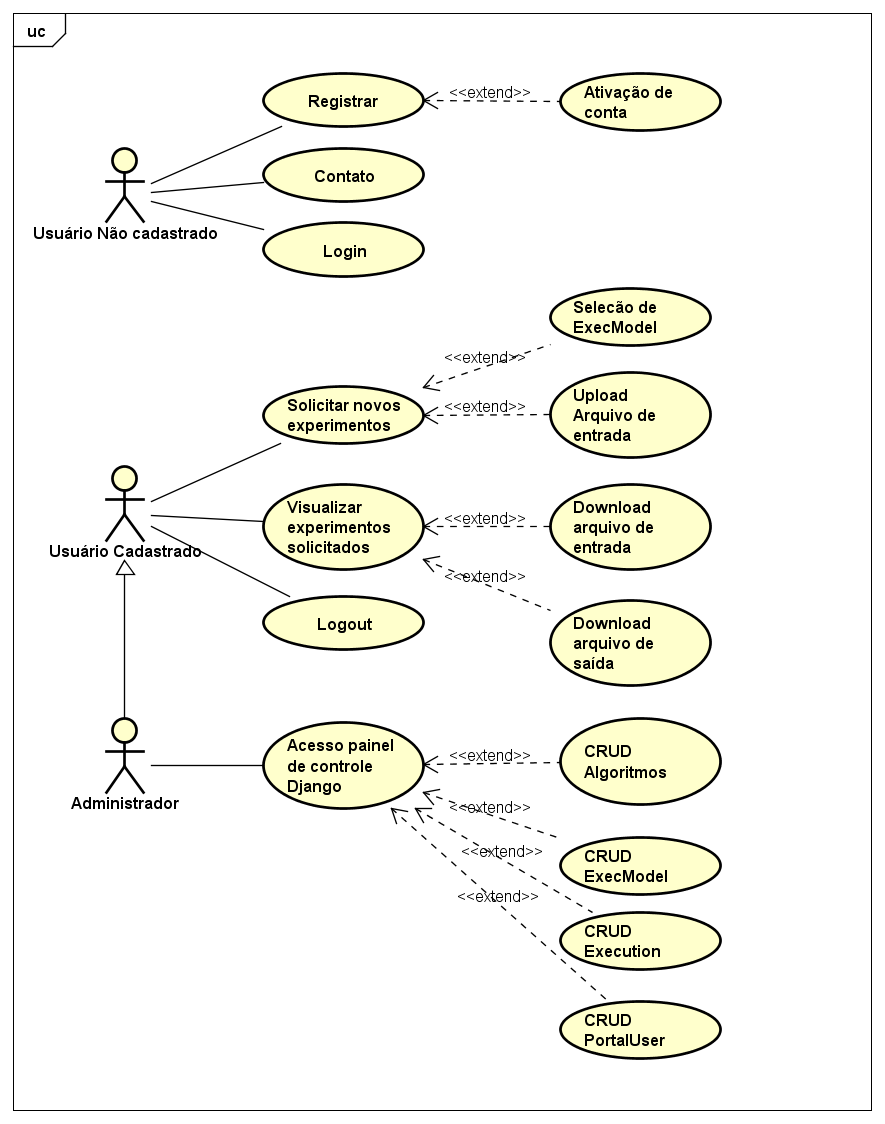
\includegraphics[width=1\textwidth]{UseCase_tg}
	\caption{
		Diagrama de casos de uso do projeto.
	}
	\label{fig:usecase}
\end{figure}

As funcionalidades do sistema podem ser divididas em 3 grupos distintos (Figura \ref{fig:usecase}).
\subsection{Usuário Anônimo}
Um usuário anônimo possui a permissão de acessar áreas de informação a respeito do sistema, de contato com o administrador do sistema, e da área de registro, onde pode solicitar o registro e, seguindo as orientações apresentadas, fazer login como um usuário registrado. (Figura \ref{fig:userstory4})
\subsection{Usuário registrado}
O usuário registrado tem permissão de criar execuções no portal, para isso ele faz o \emph{upload} de um arquivo que será utilizado como entrada no algoritmo selecionado. O usuário também pode monitorar o estado dos execuções que ele requisitou e fazer o \emph{download} dos arquivos de cada experimento, tanto o arquivo de entrada, como a saída~(se houver) do algoritmo. O usuário pode selecionar execuções realizadas por ele e as excluir. (Figura \ref{fig:userstory3})
\subsection{Administrador}
O administrador tem as mesmas capacidades do que um usuário registrado e detém privilégios de acesso ao painel de administração do Django. Isso permite que ele faça o cadastro de novos algoritmos no sistema e a editar qualquer informação que o sistema detenha no banco de dados. (Figura \ref{fig:userstory2})


\section{Modelos de dados}
\begin{figure}
	\centering
	\begin{minipage}[c]{1\textwidth}
		\begin{lstlisting}[language=Python, frame=single]
from django.db import models
from django.contrib.auth.models import User


class Algorithms(models.Model):
	idAlg = models.AutoField(primary_key=True)
	nameAlg = models.CharField(null=False, blank=False, max_length=100)
	desc = models.CharField(null=True, blank=False, max_length=500)
	command = models.CharField(null=False, blank=False, max_length=100)

	def __unicode__(self):
		return self.nameAlg


class UsuarioPortal(models.Model):
	nickname = models.CharField(
		default='default', max_length=30, blank=False, null=True)
	company = models.CharField(
		default='default', max_length=50, blank=False, null=True)
	usuario = models.OneToOneField(User)
	date_register = models.DateTimeField('date_register', auto_now_add=True)
	last_access = models.DateTimeField('last_access', auto_now=True)
	resultsPerPage = models.IntegerField(default=10)

	def __unicode__(self):
		return self.nickname


def user_directory_path_in(instance, filename):
	return './users/user_{0}/{1}/input'.format(instance.request_by.usuario.id, instance.id)


def user_directory_path_out(instance, filename):
	return './users/user_{0}/{1}/output'.format(instance.request_by.usuario.id, instance.id)


class Execution(models.Model):
	request_by = models.ForeignKey(UsuarioPortal)
	date_requisition = models.DateTimeField(
		'date_requisition', auto_now_add=True)
	status = models.IntegerField(default=1)
	algorithm = models.ForeignKey(Algorithms, null=True, blank=False)
	inputFile = models.FileField(upload_to=user_directory_path_in, null=True)
	outputFile = models.FileField(upload_to=user_directory_path_out, null=True)
	time = models.FloatField(default=-1)
	
	def __unicode__(self):
		return self.request_by.id
		\end{lstlisting}
		\clearpage
		\caption{
			Models.py
		}
		\label{fig:modelo}
	\end{minipage}
\end{figure}
Definidas as funcionalidades a serem desenvolvidas, foram criados modelos de dados para manter as informações dos usuários, de algoritmos disponíveis pelo sistema e execuções requisitadas pelos usuários.

Essas 3 classes compõem o modelo de dados (Figura \ref{fig:classdiagram}) que integram todas as funcionalidades do sistema, todos herdam a base de modelo do Django. Uma visão mais detalhada dos modelos pode ser observada na Figura \ref{fig:modelo}, o arquivo desenvolvido para definir os modelos do sistema.


\subsection{Algorithm}
Essa classe é responsável por manter os dados referentes ao(s) algoritmo(s) que o sistema disponibiliza, é composto por 3 atributos que representem o nome do algoritmo, a descrição de seu propósito, e o comando que deverá ser utilizado para executá-lo.

\subsection{Execution}
A classe \emph{Execution} mantém todas as informações referentes a uma execução. Ela inclui uma chave estrangeira que referencia o usuário que requisitou-a, a data na qual a requisição foi feita, o status da execução, outra chave estrangeira que referencia qual algoritmo será utilizado, dois campos para os endereços nos quais devem ser mantidos os dados de entrada e saída à serem usados, e o tempo gasto na execução.

\subsection{PortalUser}
O PortalUser é a classe que mantem os dados de cada usuário do portal. Ela se relaciona com a aplicação nativa do Django para autenticação de usuários, a "\emph{Auth}", que continua tratando das tarefas relacionadas a acesso ao sistema. Essa aplicação mantém os dados de usuário, senha, \emph{e-mail} e informações de data de registro e último acesso.

Além disso, a classe portal mantém outros dados:
\begin{itemize}
	\item Nickname (Utilizado para mensagens de contato e alertas pelo sistema).
	\item Company (Para manter os dados de qual instituição o usuário pertence).
	\item ResultsPerPage (Preferência de quantos resultados por página o usuário deseja quando for visualizar sua lista de execuções).
\end{itemize}

\begin{figure}
	\centering
	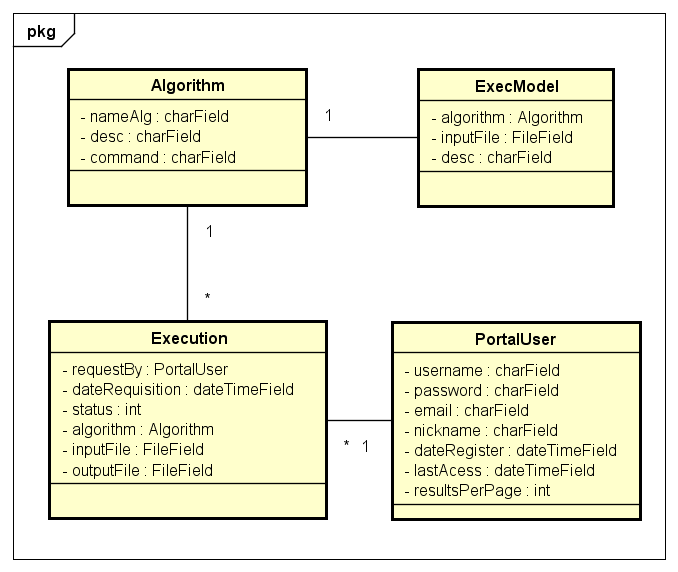
\includegraphics[width=1\textwidth]{class_diagran_tg}
	\caption{
		Diagrama de classes da aplicação.
	}
	\label{fig:classdiagram}
\end{figure}

\section{Fluxo de execução}

\begin{figure}
	\centering
	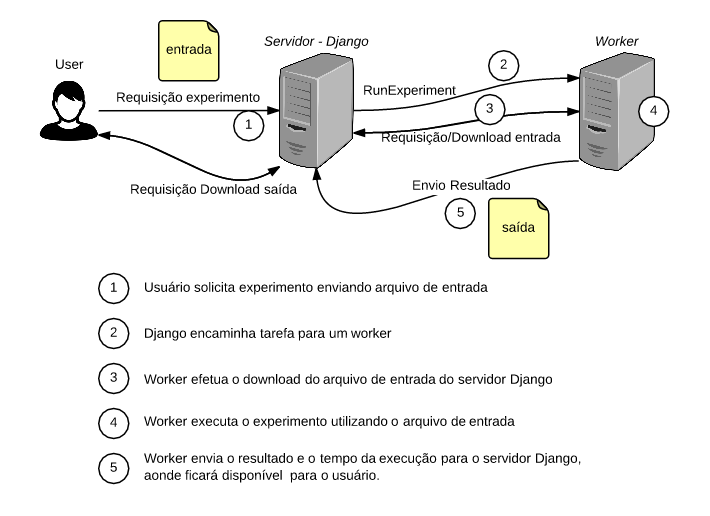
\includegraphics[width=1\textwidth]{diagrama}
	\caption{
		Fluxograma.
	}
	\label{fig:diagrama}
\end{figure}

O fluxo de execução do portal segue conforme a Figura \ref{fig:diagrama}.

\section{Etapas de implementação}
Essa seção irá explorar problemas e as soluções utilizadas no desenvolvimento de algumas funcionalidades do portal.
\subsection{Formulário de Contato}
A página de contato do sistema foi desenvolvida utilizando um formulário que exige informações necessárias para identificação e endereço de resposta de quem efetuou o contato. Para isso foi utilizada a aplicação \emph{django-crispy-forms} para obtenção e validação de dados.

\subsubsection{Django Crispy Forms}
Durante a implementação dessa funcionalidade foi instalada a aplicação Crispy. Ela trata da criação de formulários e executa a validação e renderização desses formulários. Quando um usuário preenche incorretamente um formulário, ela trata de renderizar um novo fazendo alterações nos campos preenchidos incorretamente, tornando evidente aonde se encontram os erros de preenchimento.

Esse \emph{third-party-package} foi utilizado não somente na tarefa de contato como também em todos os demais formulários do projeto.

\subsection{Registro de Usuário}


Como qualquer pessoa deve poder utilizar o portal, é imprescindível que haja uma forma autônoma de registro de novos usuários. No primeiro momento tentou-se implementar a funcionalidade utilizando formulários e verificações desenvolvidas no próprio projeto, mas durante o desenvolvimento foi encontrada uma solução mais rápida e mais adequada, o uso do \emph{third-party-package "Django-Registration-Redux"}.

O \emph{Django-Registration-Redux} provê as funcionalidades de registro de usuários para projetos Django. Essa aplicação já dispõe de templates e formulários para desempenhar a sua função, também contém um sistema de ativação de contas no qual o usuário que solicitou registro recebe um e-mail no endereço usado no cadastro que contém um link para ativar sua conta, forçando uma verificação de que o e-mail utilizado existe e pertence mesmo ao usuário.

Por padrão ela mantém apenas os dados de \emph{e-mail}, nome e senha do usuário que solicitou o registro, o que satisfaz os requisitos mínimos para executar sua funcionalidade, porém para o sistema em desenvolvimento, pareceu interessante a possibilidade de obter mais dados do usuário em seu cadastro, tais como instituição a qual o usuário pertence (Universidade, empresa, etc.), apelido pelo qual o usuário opta por ser tratado, e outras informações que podem ser úteis posteriormente ao administrador do sistema.

Além disso, essa aplicação não tem por padrão, nenhuma forma de filtro de domínios de endereços de e-mail, o que também pode ser útil ao sistema, caso o administrador queira limitar o acesso do portal aos usuários que detenham um e-mail de um domínio específico.
\begin{figure}
	\centering
	\begin{subfigure}[c]{1\textwidth}
		\begin{lstlisting}[language=Python, frame=single]
from django import forms
from registration.forms import RegistrationFormUniqueEmail
from .models import Algorithms


class UsuarioPortalForm(RegistrationFormUniqueEmail):
	nickname = forms.CharField(required=False)
	company = forms.CharField(required=False)
	\end{lstlisting}
		
		\caption{forms.py}
		\label{fig:formRegister}
	\end{subfigure}
	
	\begin{subfigure}[c]{1\textwidth}
		\begin{lstlisting}[language=Python, frame=single]
from registration.backends.default.views import RegistrationView
from experiment.forms import UsuarioPortalForm
from experiment.models import UsuarioPortal
		
class MyRegistrationView(RegistrationView):
	
	form_class = UsuarioPortalForm
	
	def register(self,request,form_class):
		new_user = super(MyRegistrationView,self).register(request, form_class)
		user_profile = UsuarioPortal()
		user_profile.usuario = new_user
		user_profile.nickname = form_class.cleaned_data['nickname']
		user_profile.company = form_class.cleaned_data['company']
		user_profile.save()
		return user_profile
			\end{lstlisting}
		
		\caption{regbackend.py}
		\label{fig:view}
	\end{subfigure}
\end{figure}

Para desenvolver essas ideias, foi criado um formulário com os campos extras desejados que estende o formulário padrão do \emph{Django-Registration-Redux}, assim, a tela de registro de usuário(Figura \ref{fig:home}) exibe um formulário que solicita os dados tanto da aplicação, quanto do modelo de usuário. O código para criação desse formulário pode ser observado na figura(Figura \ref{fig:formRegister})
\begin{figure}
	\centering
	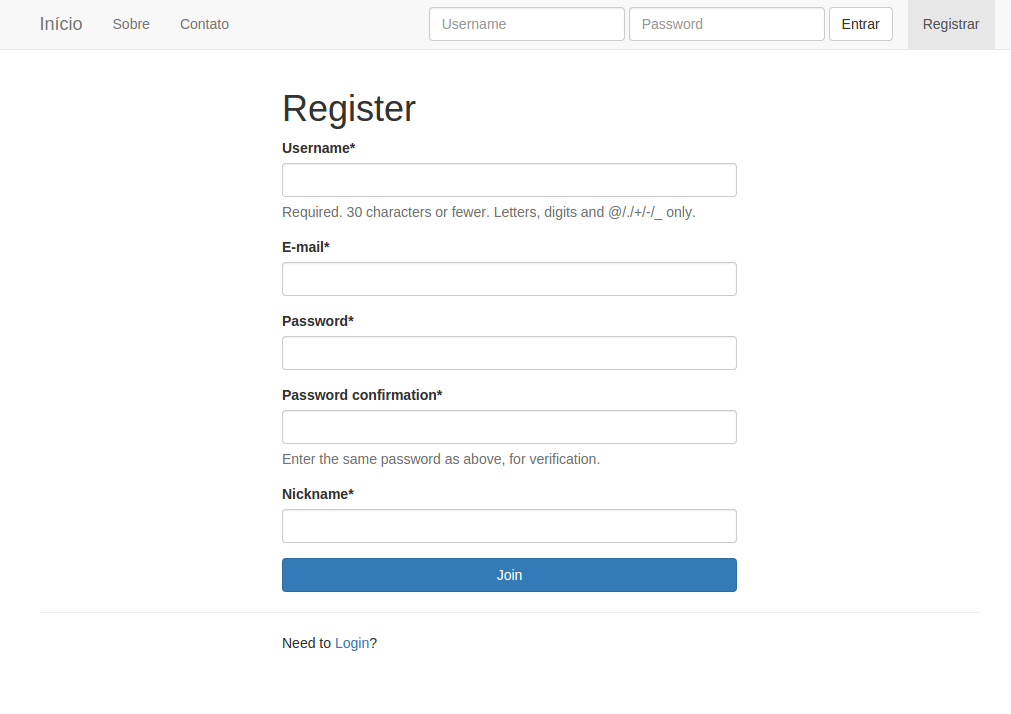
\includegraphics[width=1\textwidth]{registro}
	\caption{
		Formulário de Registro de Usuário.
	}
	\label{fig:home}
\end{figure}
Além disso, foi criada uma função para sobrescrever a função de registro no sistema, essa função continua executando a operação padrão de registro do \emph{Django-Registration-Redux}, mas também associa os dados desse registro ao dados de usuário do PortalUser. O código que realiza essa operação pode ser observado na Figura \ref{fig:view}.


\subsection{Execução remota de tarefas}
A execução remota de tarefas foi um requisito que exigiu busca de ferramentas e técnicas para sua realização. É necessário esclarecer que não é viável que o próprio processo que mantém a aplicação no ar e trata de todos os \emph{requests} realizados por usuários também lide com as execuções solicitadas pelos mesmos, pois isso causaria uma lentidão muito grande no sistema.

Para contornar esse problema foram verificadas duas técnicas: a criação de um novo processo que faria a execução do experimento, ou então o uso de alguma aplicação que gerencie filas de tarefas e distribuição das mesmas para demais processos e/ou máquinas.

Compreendida a dimensão e complexidade de criar um sistema para execução de tarefas a partir do zero, optou-se por buscar por aplicações compatíveis com as tecnologias utilizadas do projeto e que pudessem satisfazer a necessidade identificada.

A aplicação escolhida foi o Celery, ele gera filas de execução de tarefas por meio de troca de mensagens. A máquina que mantém o portal, também mantém um processo de execução do broker Redis, que faz o envio e recebimento de mensagens entre o processo que cria novas tarefas, e os \emph{workers} disponíveis para receber tarefas.

A execução de qualquer algoritmo é feita através da mesma função "RunExperiment" (Figura \ref{fig:run}). Essa função recebe como argumentos o comando que o \emph{worker} deve executar e o identificador do arquivo de entrada que deve ser utilizado. Em seguida, o \emph{worker} faz o download do arquivo de entrada para seu sistema de arquivos local e realiza a execução do algoritmo selecionado com esse arquivo de entrada recém adquirido. Entre o comando para o sistema realizar a execução, foram criadas duas variáveis para realizarem a logística de cronometrar o tempo de execução. Por fim, cria um formulário POST contendo o arquivo de saída da execução e o tempo de execução do experimento, e o envia junto com um request para a máquina que gerou a tarefa. A view para qual o request será mapeado através da url irá salvar o arquivo recebido como a saída da execução e atualizar os dados relativos a aquele experimento.

O fluxograma apresentado na Figura \ref{fig:diagrama} ilustra as operações comentadas acima, e que foram implementadas conforme mostra a código da Figura \ref{fig:run}.

\begin{figure}
	\centering
	\begin{minipage}[c]{1\textwidth}
		\begin{lstlisting}[language=Python, frame=single]
from models import UsuarioPortal, Execution
from celery.utils.log import get_task_logger
from celery.decorators import task
import requests
import os
import time

logger = get_task_logger(__name__)

@task(name="RunExperiment")
def RunExperiment(execution, ide):
	os.system("mkdir " + str(ide))
	os.system("wget http://10.1.4.28:8000/experiments/downloadInputFile?id=" +
	str(ide) + " -O ./" + str(ide) + "/input")
	start = time.time()
	os.system(execution + " " + str(ide) + "/input >" + str(ide) + "/output")
	dur = time.time() - start
	files={'file': str("/"+str(ide) + "/output")}
	path = str(str(ide)+"/output")
	files = {'file': open(path, 'rb')}
	data = {'id':str(ide),'time':dur}
	r = requests.post('http://10.1.4.28:8000/experiments/result', files=files,data=data)
	print (r.status_code, r.reason)
		\end{lstlisting}
		\caption{
			tasks.py
		}
		\label{fig:run}
	\end{minipage}
\end{figure}


Essa implementação permite ao portal criar tarefas que serão executadas pelos chamados \emph{workers}. Os \emph{workers} são processos independentes que devem ser iniciados nas máquinas que irão executar o processamento dos algoritmos e que trocam mensagens com o sistema que solicitou a execução.


\subsection{Acompanhamento de execuções}



Após a requisição de uma execução, os dados a respeito da mesma são adicionados a uma tabela (Figura \ref{fig:funcional}) contendo todas as execuções solicitadas por aquele usuário, e ficam disponíveis na tela inicial do portal. É através dessa tabela que o usuário pode interagir com as execuções requisitadas. Através da tabela, é possível efetuar o \emph{download} do arquivo de entrada e de saída (se houver) da execução. Além disso o usuário tem a opção de selecionar e excluir os dados referentes a execuções que ele solicitou.

Além dos dados gerados na requisição da execução, são apresentados outros 2 dados que informam a situação e o tempo da execução, são eles:
\begin{figure}
	\centering
	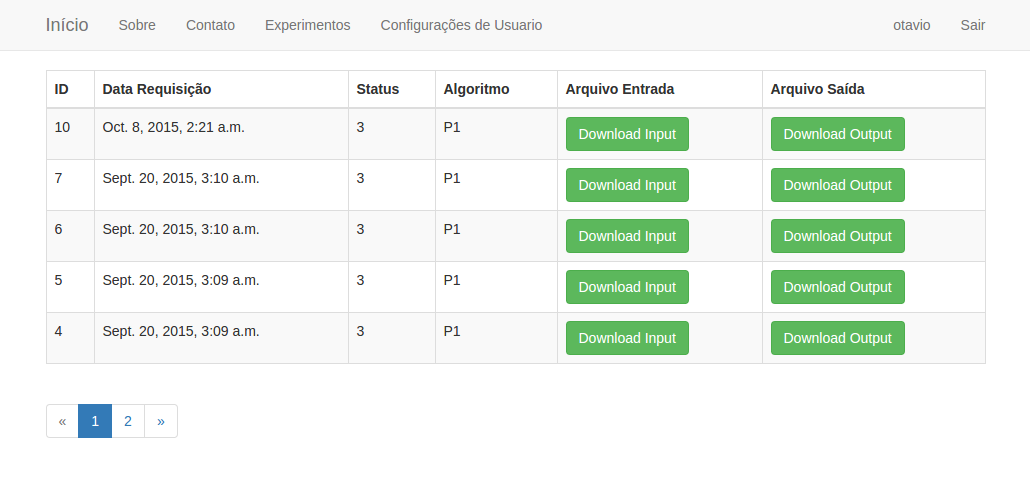
\includegraphics[width=1\textwidth]{userhome}
	\caption{
		Tela de acompanhamento das execuções.
	}
	\label{fig:funcional}
\end{figure}
\begin{itemize}
	\item Tempo: Representando quanto tempo foi gasto na execução.
	\item Status: Informa ao usuário se a execução já foi processada ou se ainda está aguardando um \emph{worker} assumir a tarefa.
\end{itemize}


\subsection{Sistema de arquivos}

Como as tarefas realizadas pelo portal exigem dados para serem processados pelo algoritmo, e gera novos dados, foi necessário criar um sistema de arquivos para manter uma ordem na qual seja possível recuperar esses arquivos após o seu processamento.
O sistema foi implementado conforme a Figura  \ref{fig:filesystem} ilustra. Nele, é escolhido um diretório como sendo a raiz de todos os arquivos que o portal irá manter referente a dados de entrada e saída dos algoritmos, e esses dados serão mantidos em diretórios nomeados de acordo com o identificador do experimento ao qual pertencem, e esse diretório, por sua vez, será mantido em um outro diretório nomeado de acordo com o identificador do usuário que requisitou o experimento.

\begin{figure}
	\centering
	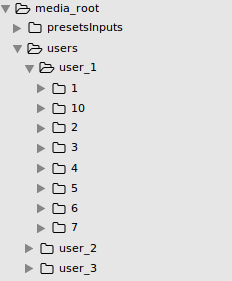
\includegraphics[width=0.7\textwidth]{filesystem}
	\caption{
		Sistema de Arquivos.
	}
	\label{fig:filesystem}
\end{figure}

\chapter{Resultados}
Ao término do trabalho, foi criado um modelo que satisfaz os requisitos levantados durante a fase de planejamento do portal. Através do modelo gerado, a comunidade de pesquisadores/desenvolvedores de novos algoritmos pode disponibilizar a utilização dos mesmos para qualquer pessoa.

Além disso, o modelo gerado foi utilizado para a criação de um portal que realiza a execução da versão \emph{n}*log(\emph{n}) e paralela do \emph{Friends-of-Friends}, tornando agora possível que pesquisadores utilizem o algoritmo para encontrar soluções baseadas em seus próprios conjuntos de dados e verifiquem a diferença de desempenho entre execuções utilizando diferentes algoritmos e/ou entradas. O portal em questão foi executado utilizando duas máquinas disponíveis no Laboratório de Sistemas de Computação (LSC) da UFSM, uma delas mantém o sistema Django disponibilizando o acesso e principais funcionalidades do portal, e a outra age como o único \emph{worker} do sistema, executando as tarefas que o portal gera.

Os teste submetido ao portal para verificar a exatidão e consistência das operações consistiu em executar o algoritmo selecionado utilizando um certo conjunto de dados de entrada, e comparar seu resultado com uma execução feita manualmente utilizando o mesmo algoritmo e o mesmo conjunto de dado. O conjunto de dados de saída processados por ambas as execuções (manual e intermediada pelo portal) resultaram em arquivos completamente iguais, satisfazendo o teste.

\chapter{Conclusão e Trabalhos Futuros}
O trabalho conseguiu satisfazer os requisitos propostos, gerando um modelo de projeto Django que permite que seus usuários executem algoritmos de alto desempenho produzindo resultados disponibilizados no próprio projeto, além de uma medição do tempo de execução que não sofre interferência de disputa por recursos da máquina que mantém o projeto.

Como trabalho futuro, surgiu a ideia de utilizar a ferramenta de virtualização de ambiente "Docker", para criar um método mais prático de distribuição desse modelo.

\setlength{\baselineskip}{\baselineskip}
\bibliographystyle{abnt}
\bibliography{../graphics,../languages}

\end{document}
